\chapter{Kompilace programu}
\label{chap:kompilace}
\section{Git}
Tato dokumentace spolu se zdrojovými kódy programu je veřejně dostupná na:
\begin{center}
	\texttt{https://bitbucket.org/Quimby/solar/src}
\end{center}
Popřípadě přímo stažitelná pomocí git:
\begin{center}
\texttt{git clone https://bitbucket.org/Quimby/solar.git}
\end{center}
Po kompilaci se u spustitelných souborů objeví obě dokumentace a také jeden příklad vstupního souboru pro \texttt{FormattedFileParser} a jedna zaznamenaná simulace.
\section{Windows}
Ve složce \texttt{buildVS/} je předpřipravený .sln projekt pro Visual Studio 2015 Community Edition, který by měl obsahovat vše potřebné pro správné zkompilování. Druhou možností je stejně jako na Unixu vytvořit si vlastní projekt pomocí programu \textbf{CMake}.
\section{Unix}
Ke kompilaci je potřeba mít nainstalován balíček \texttt{xorg-dev}(vyžaduje ho GLFW, viz. \cite{GLFW}). Dále jsou potřeba programy \textbf{CMake, make} a nějaký kompilátor, který \textbf{CMake} pozná - např. \textbf{g++}. Poté by mělo stačit pustit následující sekvenci příkazů:
\begin{lstlisting}
cd <složka se staženými soubory(obsahuje CMakeLists.txt)>
mkdir build
cd build/
#případně Debug
cmake .. -DCMAKE_BUILD_TYPE=Release 
make
\end{lstlisting}
Což by mělo vytvořit složku \lstinline|build/bin/| s potřebnými soubory. Také zde je připravena složka \texttt{buildUbuntu/} která obsahuje předem vytvořený makefile, ale nevím kde všude bude funkční.
\chapter{Uživatelská příručka}
\label{chap:userGuide}
\section{Požadavky}
Vyžaduje verzi OpenGL 3.3 nebo vyšší a rozšíření  \texttt{GL\_ARB\_clip\_control} nebo \texttt{GL\_NV\_depth\_buffer\_float}. Jinými slovy by program měl snad fungovat na většině dnešní počítačů s aktuálními grafickými ovladači( výjimkou by mohli být starší integrované grafiky od Intelu). Ke spuštění \texttt{.exe} na Windows je navíc potřeba balíček Microsoft Visual C++ 2015 Redistributable - aktuální verze na \url{https://www.microsoft.com/cs-CZ/download/details.aspx?id=53840}.
Také v případě grafického výstupu(který se zapne jako výchozí) je doporučená velikost okna minimálně 1000x500 pixelů.
\section{Základní ovladání}
Při spuštění se program otevře v výchozím grafickém režimu, kde dojde k nahrání zabudované Sluneční soustavy. Simulace se ovládá pomocí grafického rozhraní, které je popsáno na následující okomentované sadě obrázků. Snaha byla, aby tato sekce nemusela existovat a uživatelské rozhraní bylo dostatečně intuitivní samo o sobě. Proto je šance, že při najetí myší na většinu grafických prvků se zobrazí doplňující popis. Kamera se ovládá pomocí myši:
\begin{description}
	\item \textbf{levé tlačítko} otáčení kamery okolo svého cíle
	\item \textbf{pravé tlačítko} pohyb kamery do stran
	\item \textbf{ALT + levé tlačítko} rozhlížení do stran
	\item \textbf{Kolečko} přibližování a oddalování cíle
	\item \textbf{ALT + kolečko} pohyb dopředu/dozadu.
\end{description}
\begin{landscape}
\begin{figure}[ht]
	\caption{Grafické rozhraní programu}
	\centering
	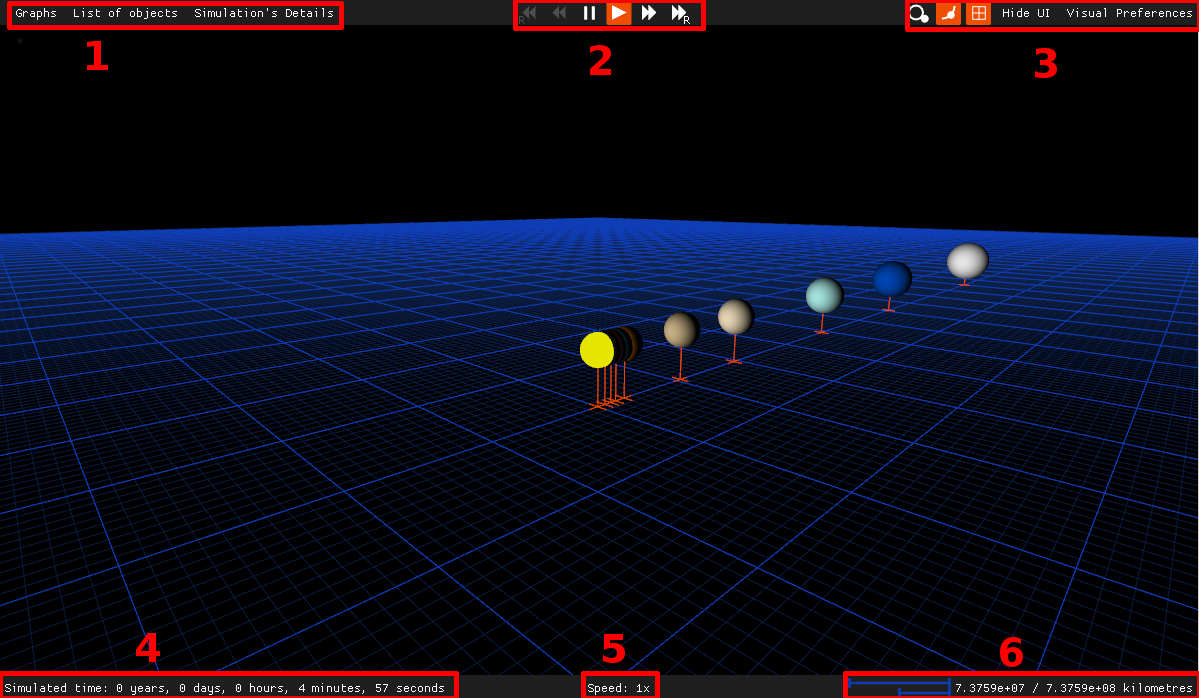
\includegraphics[width=\linewidth,keepaspectratio]{Figs/Overview}\\
	\textit{1. Tlačítka s jednotlivými okny. Zleva - grafy, seznam simulovaných objektů, detaily simulace}\\
	\textit{2. Ovladání simulace - zpomalení/zrychlení, zvětšení/zmenší sim. kroku a pozastavení}\\
	\textit{3. Tři přepínače zleva zapínají/vypínají - Skutečné velikosti objektů, LineTrails, vykreslování mřížky. Dále je zde tlačítko \textbf{na vypnutí} uživatelského rozhraní, které se \textbf{ znovu objeví zmáčknutím F1}. Poslední tlačítko otevře okno s nastavením grafiky. }\\
	\textit{4. Odsimulovaný čas \\ 5. Rychlost simulace vůči reálnému času.}\\
	\textit{6. Velikost menší a větší mřížky.}
\end{figure}

\begin{figure}[ht]
	\caption{Okna s detaily simulace a nastavením grafických prvků}
	\centering
	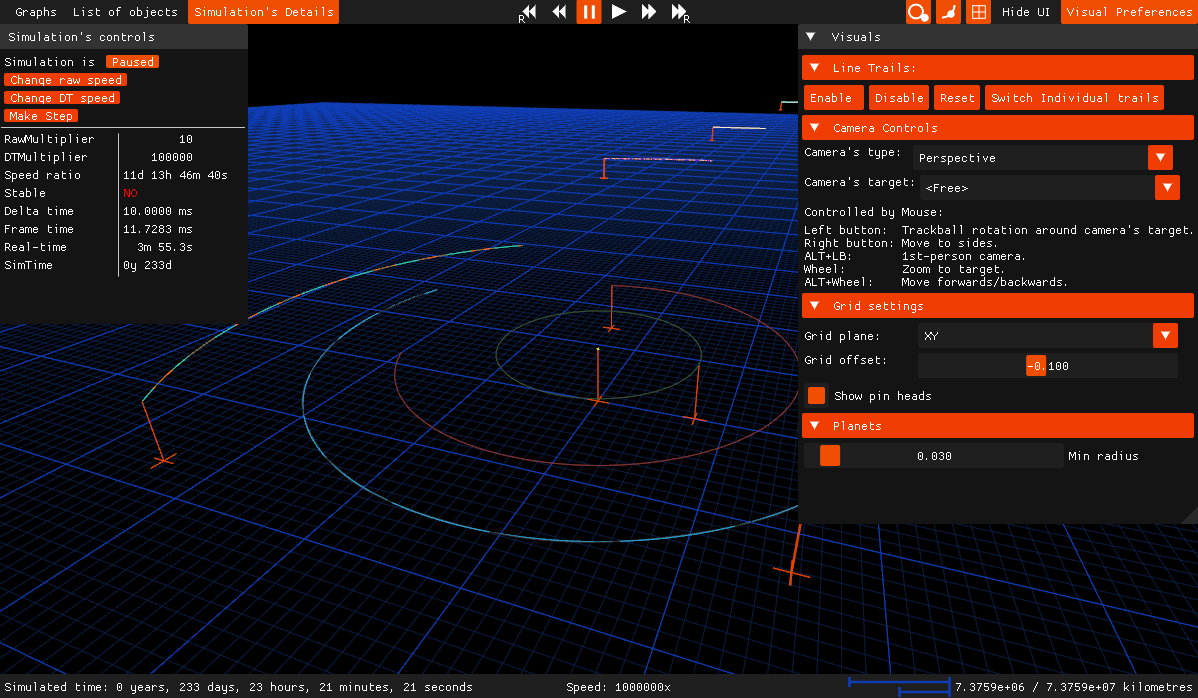
\includegraphics[width=\linewidth,keepaspectratio]{Figs/SimPropsVisualPrefs_notEdited}\\
	\textit{Levé okno nabízí pohromadě detailní informace o simulaci.\\
	Vpravo jsou pak různá nastavení. Je zde uvedeno ovládání kamery pomocí myši nebo nastavení typu kamery, orientaci mřížky a minimální velikosti objektů při vypnutí reálných velikostí.\\ Na tomto obrázku jsou reálné velikosti zapnuty a proto nejsou jednotlivé planety vůbec vidět.}
\end{figure}

\begin{figure}[ht]
	\caption{Možnosti tvorby grafů}
	\centering
	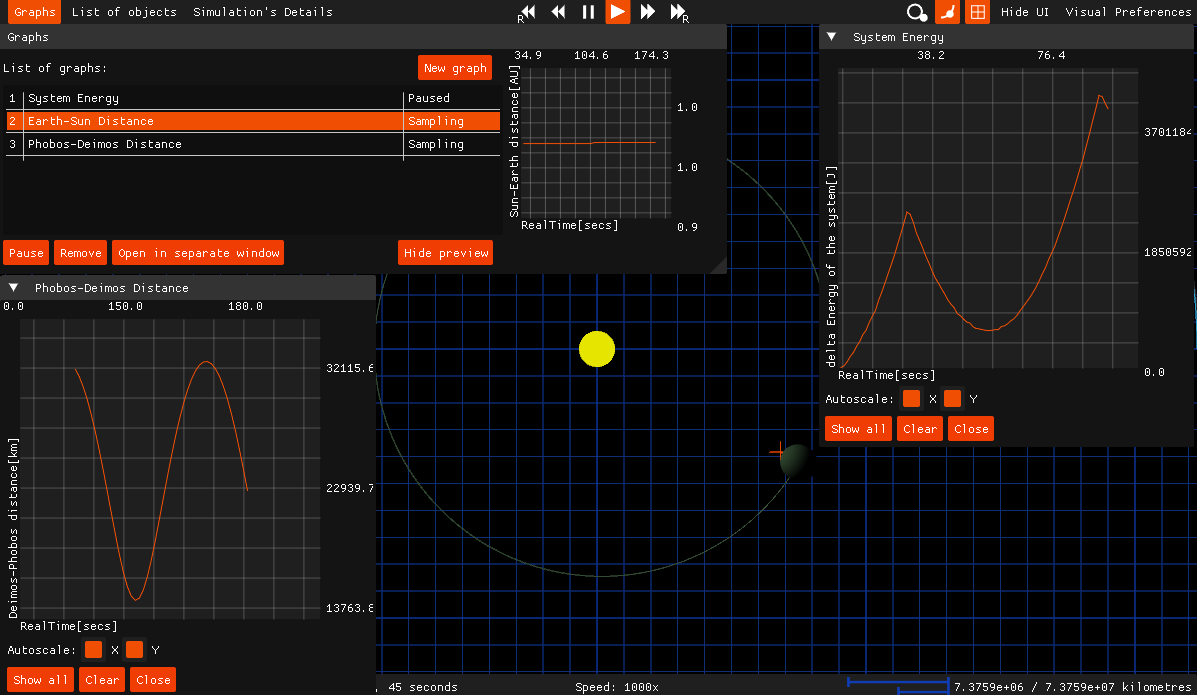
\includegraphics[width=\linewidth,keepaspectratio]{Figs/Graphs}\\
\end{figure}

\begin{figure}[ht]
	\caption{Contextové menu }
	\centering
	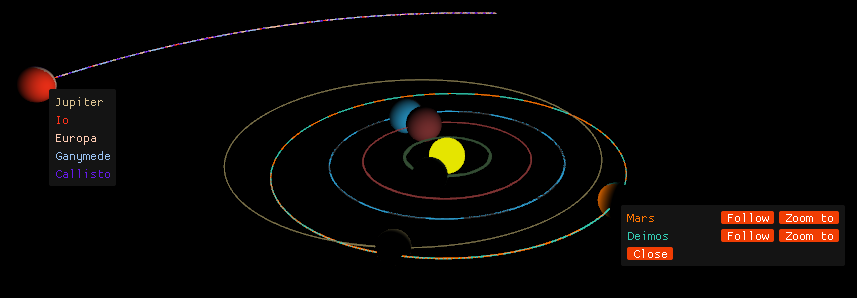
\includegraphics[width=\linewidth,keepaspectratio]{Figs/ContextMenu}\\
	\textit{Na tomto obrázku je vidět, že při najetí myši na objekty se objeví jejich jména(zde Jupiter...).\\ Při pravém kliknutí myší na objekt se otevře okno(Mars,Deimos) které navíc umožňuje zafixovat kameru na daný objekt, popřípadě se k němu přiblížit.}
\end{figure}

\begin{figure}[ht]
	\caption{Seznam simulovaných objektů}
	\centering
	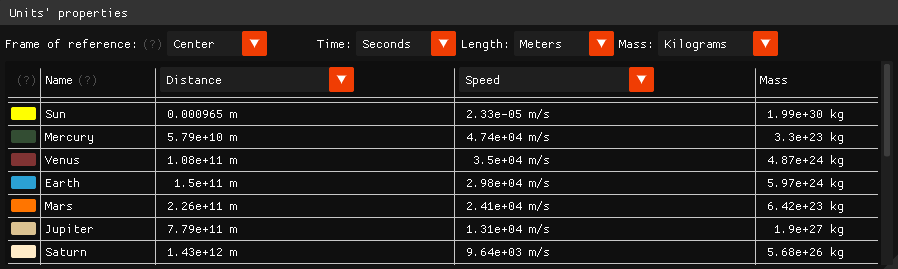
\includegraphics[width=\linewidth,keepaspectratio]{Figs/UnitsProperties_notEdited}\\
	\textit{Tento obrázek zobrazuje detail otevřeného okna se seznamem simulovaných objektů.\\ Dovoluje měřit vzájemné polohy a rychlosti všech objektů a zobrazovat je ve vybraných jednotkách.}
\end{figure}
\end{landscape}
\FloatBarrier
\section{Pokročilé možnosti}
Program také nabízí pokročilejší ovládání pomocí příkazové řádky, s níž je možné načítat simulovaná data ze souborů, vybrat si simulační metody a také možnost zaznamenat a následně přehrát uložené simulace.
Pro vypsání nápovědy a všech dostupných příkazů v českém jazyce použijte:
\ \texttt{\textbf{SolarSystem.exe -help cz}}

Vysvětlení parametrů simulace se věnuje druhá kapitola zimní dokumentace.

Uveďme zde alespoň pár dalších příkladů různých příkazů:
\begin{enumerate}
	\item \texttt{\textbf{SolarSystem.exe vstup.txt}} \\
	Načte vstupní data z formátovaného souboru \texttt{vstup.txt} a spustí simulaci, která bude běžet v reálném čase a zobrazovat se v okně 1200x700 s uživatelským rozhraním.
	\item \texttt{\textbf{SolarSystem.exe -sim -p solar -m RK4 -v win}} \\
	 Ekvivalentní zápis předchozího příkladu. S explicitním použitím modulů.
	\item \texttt{\textbf{SolarSystem.exe -sim -rm 24 -dm 3600 -x 300}} \\
	Spustí podobnou simulaci jako v 1. příkladu. Akorát bude mít 3600x větší integrační krok a bude probíhat 24x rychleji. Ve výsledku se tedy odsimuluje jeden den za jednu reálnou sekundu. Simulace se vypne po 5 minutách běhu.
	\item \texttt{\textbf{SolarSystem.exe -record -r zaznam.replay -p formatted -i vstup.txt -o vystup.txt -m semiEuler -rm 24 -dm 3600 -x 60}}\\
	Zaznamená 60 sekundovou simulaci do souboru \texttt{zaznam.replay}, vstupní data načte z formátovaného souboru \texttt{vstup.txt} a výsledná data uloží do \texttt{vystup.txt} ve stejném formátu. Simulace bude simulovat jeden den za jednu sekundu pomocí semi-implicitní Eulerovy integrační metody. Simulace se spustí v grafickém prostředí stejně jako v 1. příkladě.
	
	\textbf{POZOR:} Momentálně je možné měnit pomocí uživatelského rozhraní parametry simulace za běhu. Ovšem \textbf{nedělejte} to, nahrávací algoritmus s tím nepočítá a je to jedno z témat oprav v programátorské sekci.
	\item  \texttt{\textbf{SolarSystem.exe zaznam.replay}}\\
	Přehraje zaznamenanou simulaci z předchozího příkladu v grafickém prostředí.
\end{enumerate}
\FloatBarrier
